\documentclass{article}
\usepackage{amsmath}
\usepackage{fullpage}
\usepackage{graphicx}
\usepackage{float}
\usepackage{amssymb}
\usepackage[bottom]{footmisc}
\newcommand{\Lagr}{\mathcal{L}}
\title{Mathematics in Basketball}
\author{Tyler Lin}
\begin{document}

\maketitle
\section*{Introduction}
If you were coaching a basketball team, it seems like common sense to give your best player the majority of the shots in the game. Logically, the best player should give you the best chance of making a shot on any given possession. However, is this really the best method? What about factors like fatigue, the defense, and rhythm? Historical data from the NBA implies that a player's ability to score decreases as he is used more. With this in mind, we can explore methods to maximizing a team's scoring capability in various scenarios.
\section*{Concept}
In a basketball game, a team's possession of the ball can end with either a shot attempt, free throw attempt, or turnover by one of the five offensive players on the court (a turnover is when a player ends his/her team’s possession of the ball before they can attempt a shot e.g. stepping out of bounds, traveling, etc.).
\newline For each of the five players on a team, we can create a function $f_i$, or the efficiency function, that estimates the player's scoring effectiveness depending on his rate of use $x_i$, where $1\leq x\leq5$. In order to do so, we must determine how to quantify (a) scoring effectiveness and (b) usage rate from a player's statistics in any given season.
\subsection*{Scoring effectiveness}
To calculate the scoring effectiveness of a player $i$, we will use the simple formula $$\frac{pts_i}{poss_i}$$
where $pts_i$ represents the number of points the player scored and $poss_i$ is the number of possessions the player ended, defined as $$ poss_i = \text{shot attempts + 0.44\footnotemark
(free throw attempts) + turnovers}.$$ In essence, this formula calculates a player's points per possession (PPP), or the amount of points they generated over the amount of possessions they ended.
\footnotetext{\textit{Note}: 0.44 is an empirically derived constant that factors in how not all free throws constitute the end of a possession (ex. technical fouls), so it is used instead of 0.5.}
\newpage\subsection*{Usage rate}
To calculate a player's usage rate, we will use the established formula
$$\frac{poss_i}{poss_{team}} \times \frac{48}{MPG_i}$$
where the subscript $team$ refers to the team's total amount of that statistic and $MPG_i=$ the minutes played per game by player $i$. This function takes the number of possessions that the player $i$ used (scaled to the full game) and divides that by the team's total possessions to calculate how often the player used a possession. Think of it as a value between 0 and 1, where 0 means the player neither attempted a shot nor committed a turnover and 1 means the player took every shot and committed every turnover for the team.
\subsection*{Graphical Representation}
A player's scoring effectiveness as a function of his usage rate over a whole season can be used as a data point. A player with multiple seasons then has multiple points that can be expressed graphically to observe his efficiency curve. In this example, I used data from Michael Jordan's career with the Chicago Bulls.
\begin{figure}[H]
\centering
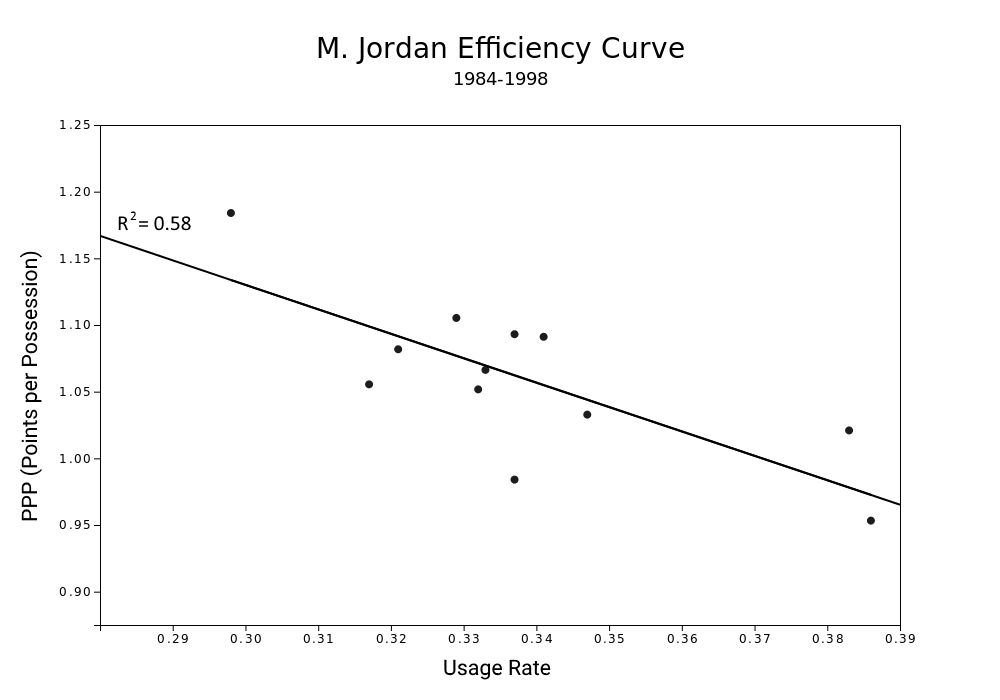
\includegraphics[width=0.75\textwidth]{jordancurve.png}
\caption{The correlation of Michael Jordan's scoring efficiency with his usage rate. Each data point represents a season of his career with the Bulls excluding the 1994-1995 season (17-game return from retirement)}
\end{figure}
It makes sense that as Jordan's usage rate increases, his efficiency would decrease. The more shots he takes, the more the defense will focus on him and try to limit his scoring. By using a linear regression as shown above, we can estimate Jordan's efficiency function to be $$f_{MJ}(x) \approx -1.83x+1.68.$$
Keep in mind that this is just a rough approximation. Players usually do not have a wide enough range of usage rates to accurately judge how their efficiency declines with use. However, using an estimate like the one above is satisfactory.
\section*{Application}
If Michael Jordan was surrounded by completely average players, how much should he be used to maximize the team's efficiency? First, let us define average. From data from the 1997-1998 NBA season (Jordan's last as a Bull), it can be determined that the average PPP of a player was $$\frac{7.9\text{ P/G}}{6.59\text{ FGA/G}+0.44(2.17\text{ FTA/G})+1.28\text{ TO/G}} = .895 \approx .9 \text{ PPP}$$
So our team consists of Michael Jordan and four players who score at a constant efficiency of 0.9 PPP. Because $f_{MJ}(0) = 1.68 >> 0.9$, a seemingly logical approach to maximizing the team's scoring output is to let Jordan shoot until his PPP decreases to the level of his teammates. In other words, on every possession the ball is given to the player with the highest chance of making the shot, which is initially Jordan. However, it turns out that this method is not ideal; if $f_{MJ}(x_{MJ}) = 0.9$, then the team's efficiency $E$ would only be 0.9 as well. Jordan would have a usage rate of almost 43 percent (which would be the highest ever), so it makes sense that the his efficiency would decline significantly.
\newline To find the true ideal usage rate for Michael Jordan, note that for a set of five players, the team's efficiency $E$ can be calculated by a weighted average of the players' efficiencies $f_1(x_1), f_2(x_2),...,f_5(x_5)$ with respect to the players' usage rates $x_1, x_2,...,x_5$: $$E=\sum_{i=1}^{5}x_if_i(x_i)$$ subject to the condition $$x_1+x_2+x_3+x_4+x_5=1.$$
We substitute Jordan's team's efficiency functions in to get 
\begin{equation*} 
\begin{split}
E & = x_1(-1.83x_1+1.68)+0.9(x_2+x_3+x_4+x_5) \\
 & = x_1(-1.83x_1+1.68)+0.9(1-x_1) \\
 & = -1.83x_1^2+0.78x_1+0.9.
\end{split}
\end{equation*}
To maximize this, we differentiate.
\begin{gather*}
\frac{dE}{dx_1} = -3.66x_1+0.78  = 0 \\
 x_1 = 0.213
\end{gather*}
which is the x-coordinate of the maximum. Then $E_{max}$ is about 0.983 PPP. 
\begin{figure}[H]
\centering
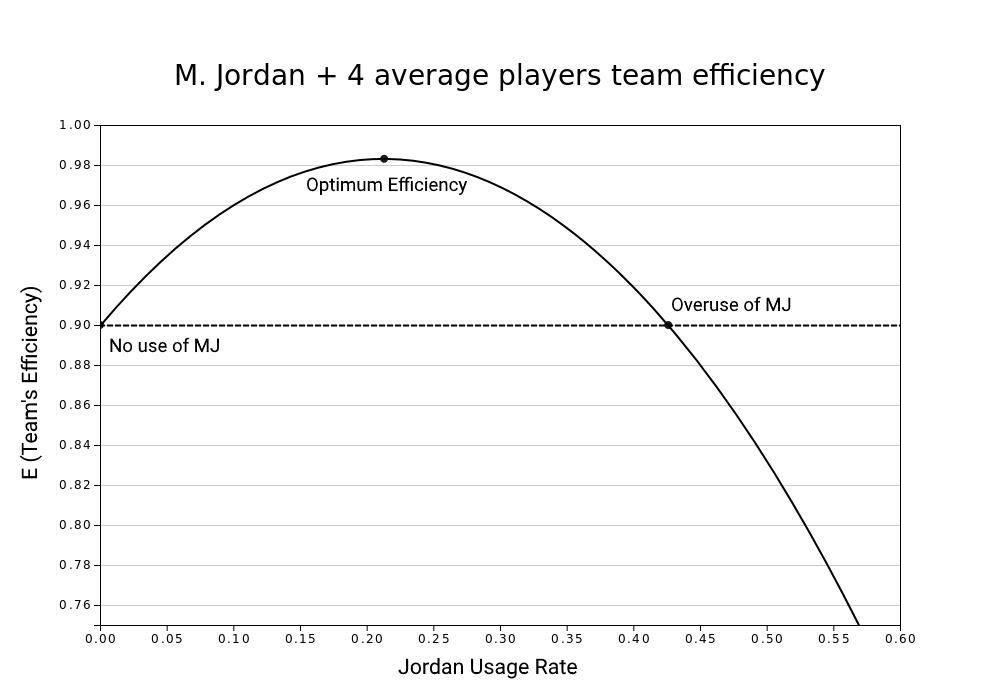
\includegraphics[width=0.75\textwidth]{team1.png}
\caption{E as a function of Jordan's usage rate.}
\end{figure}
Figure 2 illustrates an interesting result. It suggests that even if Michael Jordan was on a team with players of much lower skill than him, his usage rate should be limited to just 0.213, almost the same amount as his teammates. That's very low for a superstar like Jordan who holds the record for highest career usage percentage. However, less use of Jordan would keep the defense from honing in on just him, instead having to focus on all five players. But this is an unrealistic example. In real life, Jordan's teammates would have their own efficiency curves! Let's investigate that.
\newline We will keep the same concept, Michael Jordan surrounded by average players. This time, his teammates will be ones he actually played with. Throughout Jordan's second three-peat with the Bulls, he was joined by hall-of-famers Scottie Pippen and Dennis Rodman, who would hardly count as average. Thus we look to the next four players with the most minutes played during those three years: \textbf{Ron Harper}, \textbf{Steve Kerr}, \textbf{Toni Kukoc}, and \textbf{Luc Longley}.
\begin{figure}[H]
\centering
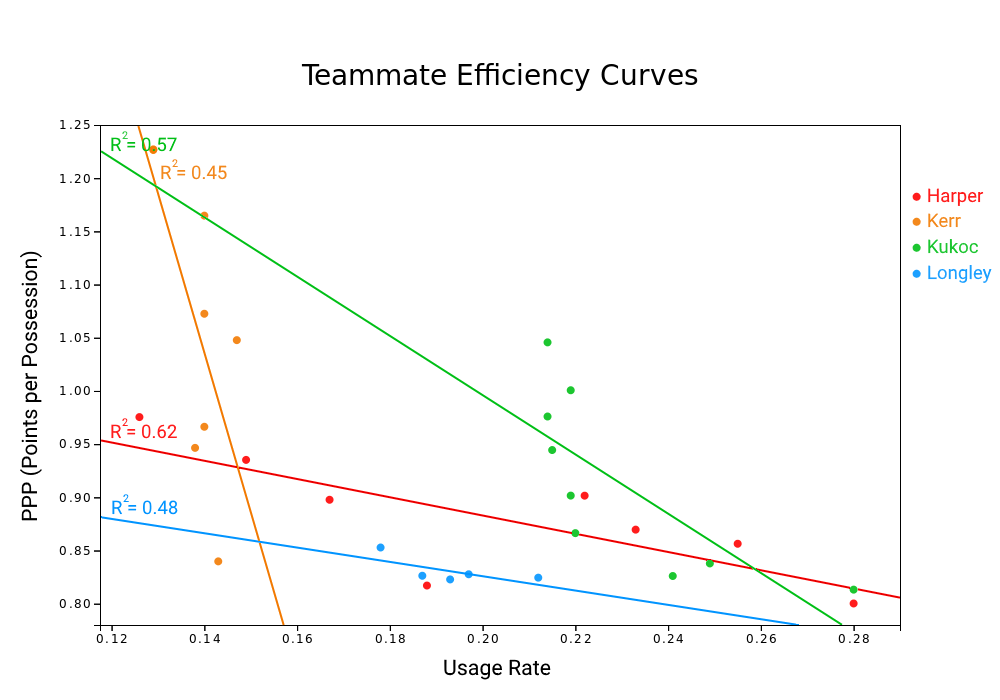
\includegraphics[width=0.75\textwidth]{harper.png}
\caption{Efficiency curves of Ron Harper, Steve Kerr, Toni Kukoc, and Luc Longley ($>48$ games played, excluded each player's first two seasons and last two seasons to account for development and decline in performance respectively).}
\end{figure}
Using linear regressions, we approximate each of the players' efficiency functions.
\begin{equation*} 
\begin{split}
 f_{RH}(x)& \approx -0.85x+1.05 \\
 f_{SK}(x)& \approx -14.91x+3.12 \\
 f_{TK}(x)& \approx -2.79x+1.56 \\
 f_{LL}(x)& \approx -0.68x+0.96
\end{split}
\end{equation*}
And Jordan's again:
$$f_{MJ}(x) \approx -1.83x+1.68$$
Let the subscripts $MJ=1$, $RH=2$, $SK=3$, $TK=4$, and $LL=5$.
We want to maximize 
\begin{gather*}
 E=x_1f_1(x_1)+x_2f_2(x_2)+x_3f_3(x_3)+x_4f_4(x_4)+x_5f_5(x_5) \\
 =-1.83x_1^2+1.68x_1-0.85x_2^2+1.05x_2-14.91x_3^2+3.12x_3-2.79x_4^2+1.56x_4-0.68x_5^2+0.96x_5
\end{gather*}
given that $$x_1+x_2+x_3+x_4+x_5=1.$$
This can be achieved by using the Lagrange multiplier technique. $$\Lagr(x_1,x_2,...,x_5,\lambda)=E-\lambda(x_1+x_2+...+x_5-1)$$
Now to find the critical points of $\Lagr$ using partial derivatives. With respect to $x_1$,
\begin{equation*}
    \begin{split}
        0&=\frac{\partial \Lagr}{\partial x_1} \\
        0&=-3.66x_1+1.68-\lambda \\
        x_1&=\frac{1.68-\lambda}{3.66}.
    \end{split}
\end{equation*}
Using the same process, we eventually get $$x_2=\frac{1.05-\lambda}{1.7}\text{, } x_3=\frac{3.12-\lambda}{29.82}\text{, } x_4=\frac{1.56-\lambda}{5.58}\text{, and } x_5=\frac{0.96-\lambda}{1.36}.$$
By substituting these values into the optimization condition, one can calculate $\lambda$.
$$\frac{1.68-\lambda}{3.66}+\frac{1.05-\lambda}{1.7}+\frac{3.12-\lambda}{29.82}+\frac{1.56-\lambda}{5.58}+\frac{0.96-\lambda}{1.36}=1$$
$$\lambda = 0.653$$
It is now possible to determine each player's optimal usage rate and respective efficiency along with the team's maximum efficiency.
\begin{table}[h]
 \centering
 \begin{tabular}{|c||c c c c c|} 
 \hline
  & Jordan & Harper & Kerr & Kukoc & Longley \\ [0.5ex] 
 \hline\hline
 USG Rate & \textbf{0.28} & 0.24 & 0.09 & 0.16 & 0.23 \\ [1ex] 
 \hline
 PPP & 1.17 & 0.84 & 1.88 & 1.12 & 0.80 \\ [1ex] 
 \hline
\end{tabular}
\end{table}
\newline $$E_{max}=0.28(1.17)+0.24(0.84)+0.09(1.88)+0.16(1.12)+0.23(0.80)=1.06 \text{ PPP}$$
It turns out that in this case, Jordan's optimal usage rate is 0.28 - higher than the other scenario, but still much lower than one would think. In fact, a 0.28 usage rate would be the lowest of his whole career! Nonetheless, limiting Jordan's shots in this situation is required to achieve maximum team efficiency. Even if Jordan's teammates were much less talented than him, appropriating a fair enough amount of use to them helps to keep the defense honest, which in turn may open up holes for Jordan to exploit. The effects of this can be seen if we calculate Jordan's theoretical points per game in this scenario. Knowing that the Bulls averaged 89 possessions per game in the 1997-98 season, Jordan's PPG would be
$$89 * 0.28 * 1.17 = 29.2,$$ which is actually \textit{higher} than his actual PPG that season of 28.7!
\section*{Conclusion}
Keep in mind that these findings should by no means be taken as concrete. Many assumptions were made, as basketball is an ever-changing and unpredictable sport. One of these assumptions is that efficiency curves are linear. They could be more quadratic or even cubic, but the data gathered in the scenarios supported linear regressions. Nevertheless, our results may hold some value. They suggest that using the play that has the highest probability of success on each possession is not ideal - instead, a coach should focus on maximizing the overall efficiency of a team by distributing usage in a holistic manner.
\section*{References}
Skinner, Brian. "The Price of Anarchy in Basketball." \textit{Journal of Quantitative Analysis in Sports}, 
     vol. 6, no. 1, 28 Jan. 2010. 
\newline http://www.math.harvard.edu/archive/21a\_spring\_09/PDF/11-08-Lagrange-Multipliers.pdf
\newline https://www.basketball-reference.com/about/glossary.html
\end{document}
